\section{The Discovery of the Gluon \cite{gluon}}
The gluon was discovered by the measurement of three jet events at the $e^+e^-$ collider PETRA. It was the first confirmation of the quantum chromodynamic (QCD) and also the first discovered gauge boson after the photon.
\subsection{Historical Context}
Around 1954 the developement of the QCD and the Yang-Mills theory started. Together, both theories build the fundament of the formulation of the gauge theories of the weak and strong interaction.
In 1964 Murray Gell-Mann and George Zweig brought up the quark hypothesis. It was the first time that quarks were mentioned as components of hadrons. But at this point, it was still unclear which force binds the quarks into hadrons and if quarks could also be free. If this force is caused by a new interaction there would also be the possibility of having a new exchange particle. Beside this idea there was the experimental evidence that the wavefuntion of the fermion $\symup{\Delta}^{++}$ is symmetric under the exchange of two quarks. This was in disagreement with the Pauli principle which suggests that fermion wavefuntions need to be antisymmetric. Oscar W. Greenberg fixed that problem by postulating another quantum number, \textbf{Colour}, in 1964. The colour could appear in three different states \textit{red}, \textit{blue}, \textit{green} and their anti versions. Together with the colour wavefuntion the total wavefunction of the baryon was again antisymmetric. An experimental indication for this three colours was given by the ratio between the cross section of $e^-e^+$ into two quarks and two muons. The experimental results showed a missing factor of $3$ in the theoretical prediction.
The results from electron-proton scattering at the Stanfort Linear Accelerator Center (SLAC) indicated that just \SI{50}{\percent} of the total proton momentum was carried by quarks. This interpretation was done by Chris Llewellyn-Smith in 1968 and was the first indication for the gluon. In 1973 David Politzer, David Gross and Frank Wilczek formulated the QCD as an $\text{SU}(3)_{\text{colour}}$ group with the gluon as gauge boson corresponding to the interaction. In 1975 the $e^-e^+$ collider SPEAR at SLAC provided the first measurements of two jet events ($e^-e^+ \to q\bar{q}$). In the following year John Ellis, Graham Ross and Mary Garllard formulated the possibility of gluon production through bremsstrahlung. This process would lead to corrections for the two jet events at higher energies.\\
In 1979 the oberservation of three jet events from the TASSO collaboration at the PETRA collider at the Deutsches Elektron-Synchrotron (DESY) finally lead to the discovery of the gluon.

\subsection{Theoretical principles}
The QCD is a relativistic quantum field theory and describes the strong interaction. It is based on the $SU(3)_{\symup{C}}$ symmetry group, which leads to eight generators, the gluons. They are the gauge bosons of the QCD and mediate the strong force. Analogous to the electric charge of the quantum electrodynamic the corresponding charge of the QCD is the colour. Therefore the massless gluons couple to the colour charge of particles. Since the $SU(3)_{\symup{C}}$ is non-abelian the gluons carry colour themselves and therefore interact with each other. The gluons are vector bosons and their spin is $1$. \\
The QCD has two important characteristics emerging from the fact that the coupling constant $\alpha_S (q)$ is running. In the case of small distances between coloured particles or high momentum transfer they become asymptotically free. This phenomenon is called asymptotic freedom and gives an explanation why there is a lower energy limit for gluon bremsstrahlung. The second characteristic of the strong interaction is the colour confinement. After a specific distance between two colour-charged particles it is energetically favoured to produce two new particles besides the initial ones. This is caused by the high value of the coupling constant at long distance. Confinement is the reason that in nature just colour neutral, white, states exist. They are bounded states of colour-charged particles. More importantly for high energy physics the confiment leads to hadronization. It leads to the production of several new particles due to high energetic scattering processes. This is the reason why the initialy produced quarks will be measured as jets. The sum over the momenta of all hadrons is equal to the momentum of the initial quark.

\subsection{Experimental Setup}
The Deutsche Elektonen Synchroton (DESY) was founded at the 18.12.1959 in Hamburg.
In 1974 it was proposed to build the Positron-Elektron-Tandem-Ring-Anlage (PETRA). PETRA was completed in October 1978 and with a perimeter of \SI{2.3}{\kilo\meter} the biggest storage ring at the time. It operated at a center of mass energy between \SI{13.7}{\giga\electronvolt} and \SI{27.4}{\giga\electronvolt}. The ring includes four interaction points where the five collaborations TASSO, JADE, MARK J, CELLO and PLUTO worked. TASSO succeeded in discovering the gluon by measuring three jet events in 1979. TASSO was a \textbf{T}wo \textbf{A}rm \textbf{S}pectrometer \textbf{SO}lenoid detector. A scintillation counter, proportional chamber and a large drift chamber allowed to measure charged particles. The surrounding solenoid helped to measure the momenta more precisely. The two arms contained Cherenkov detectors and time of flight counters, which made it possible to distinguish between pions, kaons and protons.


\subsection{Measurments that lead to the Discovery}
By the time that the idea of gluon bremsstrahlung was developed, experiments started to search for events that indicate this type of bremsstrahlung. If such events existed the three jets lie in an event plane which is spanned by the three momentum vector of the initial quarks and the gluon. Sau Lan Wu made the pediction that such events would appeae at center of mass energies greater then \SI{22}{\giga\electronvolt}. In June 1979 the TASSO collaboration presented several three-jet events. But before calling it the discovery of the gluon they started to analyse their data more detailed.

\begin{wrapfigure}{l}{0.4\textwidth}
    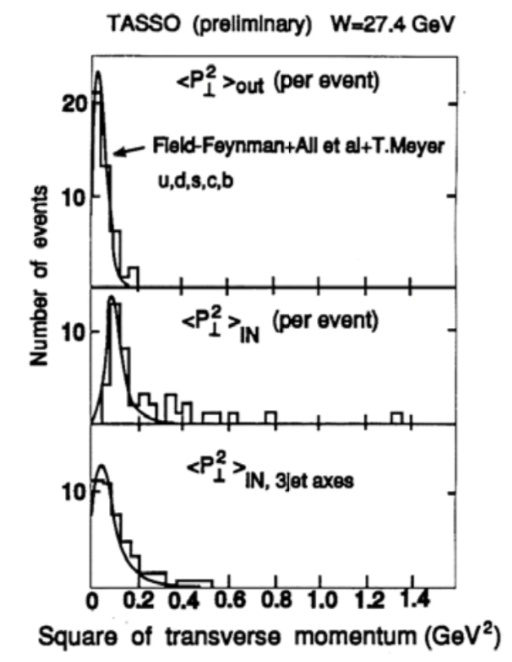
\includegraphics[width=0.38\textwidth]{graphics/pt_gluon.png}
    \caption{Comparison of $\left<p_T^2\right>_{\symup{out}}$ and $\left<p_T^2\right>_{\symup{in}}$ with the $q\bar{q}$ and the $q\bar{q}g$ model.\cite{gluon}}
  \end{wrapfigure}
  \FloatBarrier
The third jet has to come from a boson, so the first cross check made, was if it is possiple that a meson could produce such a jet.
This is not possible for a quark to emit a meson with such large momentum at the present rate. The TASSO collaboration made different measurements at energies below and above the necessary center of mass energy to produce gluon bremsstrahlung. This made it possible to study the energy dependent kinematics. In particular two different $<p_T>$ analyses have been performed. To do so a jet axis is fitted to the final state momentum of each hadronic event. In the case of $q\bar{q}$ jet production without a gluon the two jets would have the same momentum but in opposite directions. Due to this fact the contributions should cancel each other to zero in $<p_T^2>$. The energy time uncertainty causes a $<p_T^2>$ value slightly different from zero, but it is still independent from the center of mass energy. In the case of the presence of another particle the momenta would not cancel each other anymore and an asymmetry would be observed. The asymmetry would rise with higher energies. The measurements made by the TASSO collaboration indicated the later case. Other measurements at the time helped to rule out that the third jet could come from a heavier quark.
The second study already used the idea of having three jets that create an event plane. The conservation of energy and momentum allows to define two quantities $\left<p_T^2\right>_{\symup{out}}$ and $\left<p_T^2\right>_{\symup{in}}$ to characterize, how planar the event plane is. $\left<p_T^2\right>_{\symup{out}}$ is the mean squared transverse momentum normal to the plane and $\left<p_T^2\right>_{\symup{in}}$ the mean squared transverse momentum in the plane. For the case of $\left<p_T^2\right>_{\symup{out}}$ the $q\bar{q}$ model fits the data pretty well. This is also the case for $\left<p_T^2\right>_{\symup{in}}$
at low energies. But but for higher energies there appear events in the event plane, while the model does not predict them. In particular one event is predicted for $\left<p_T^2\right>_{\symup{in}} \; > \SI{0.3}{\giga\electronvolt}$ and eleven were observed. The data fit the model of a three jet event. Based on this result the possibility of three jets as a result of statistical fluctuations of the process $e^-e^+ \to q\bar{q}$ could be ruled out. Taking all this results into account this was indeed the discovery of the gluon. The discovery was confirmed by the other experiments within the following two months. \\
As a follow up the TASSO collaboration studied the spin of the gluon, to find out if the gluon is a vector boson as predicted. John Ellis and Inga Karliner predicted that the cross section depends on the so called Ellis Karliner angle. Depending on the spin of the gluon the shape of the distribution is significantly different for the gluon bein a vector boson or a scalar. The measurement showed a clear agreement with the vector boson distribution. The discovery of the gluon and the oberservation that it is indeed a vector boson lead to the confirmation of the quantum chromodynamic.
